\documentclass[12pt]{article}

\usepackage{amsmath} % بسته ضروری برای معادلات
\usepackage{graphicx} % ← این خط را اضافه کنید
\usepackage{xepersian}
\settextfont{Yas}
\setdigitfont{A Iranian Sans}

\title{تمرین Entoropy}
\author{محمد صالح علی اکبری}
\date{تاریخ تحویل 31 اردیبهشت}

\begin{document}
	
	\maketitle
	
	\section*{سؤال ۱}
		ارتباط آنتروپی با عدم قطعیت و اطلاعات در توابع پراکندگی (انتشار) و شبه آنتروپی را با رسم منحنی مربوطه تشریح کنید.
\subsection*{پاسخ}

آنتروپی مفهومی است که میزان عدم قطعیت را در یک متغیر تصادفی اندازه‌گیری می‌کند. هرچه توزیع احتمال یکنواخت‌تر باشد، آنتروپی بیشتر خواهد بود، و در نتیجه عدم قطعیت بیشتر است. آنتروپی یکی از شاخص‌های کلیدی در تحلیل پراکندگی داده‌ها است.

برای درک این موضوع، دو تابع را بررسی می‌کنیم: تابع پراکندگی (Dispersion Function) و تابع شبه آنتروپی (Entropy-like Function). این توابع برای حالتی تعریف می‌شوند که تنها دو کلاس داریم و احتمال تعلق به یک کلاس برابر با $w_1$ است.

\begin{itemize}
	\item تابع پراکندگی (آنتروپی):
	\[
	H(w) = -w_1 \log w_1 - (1 - w_1) \log (1 - w_1)
	\]
	این تابع زمانی بیشینه است که $w_1 = 0.5$ باشد. یعنی بیشترین عدم قطعیت.
	
	\item تابع شبه آنتروپی:
	\[
	f(w) = 1 - (w_1^2 + (1 - w_1)^2)
	\]
	که شکلی ساده‌تر و هموارتر برای سنجش پراکندگی است و معمولاً در الگوریتم‌هایی مانند Gini Index نیز استفاده می‌شود.
\end{itemize}

در نمودار زیر، مقایسه‌ای بین این دو تابع ارائه می‌شود:

\begin{center}
	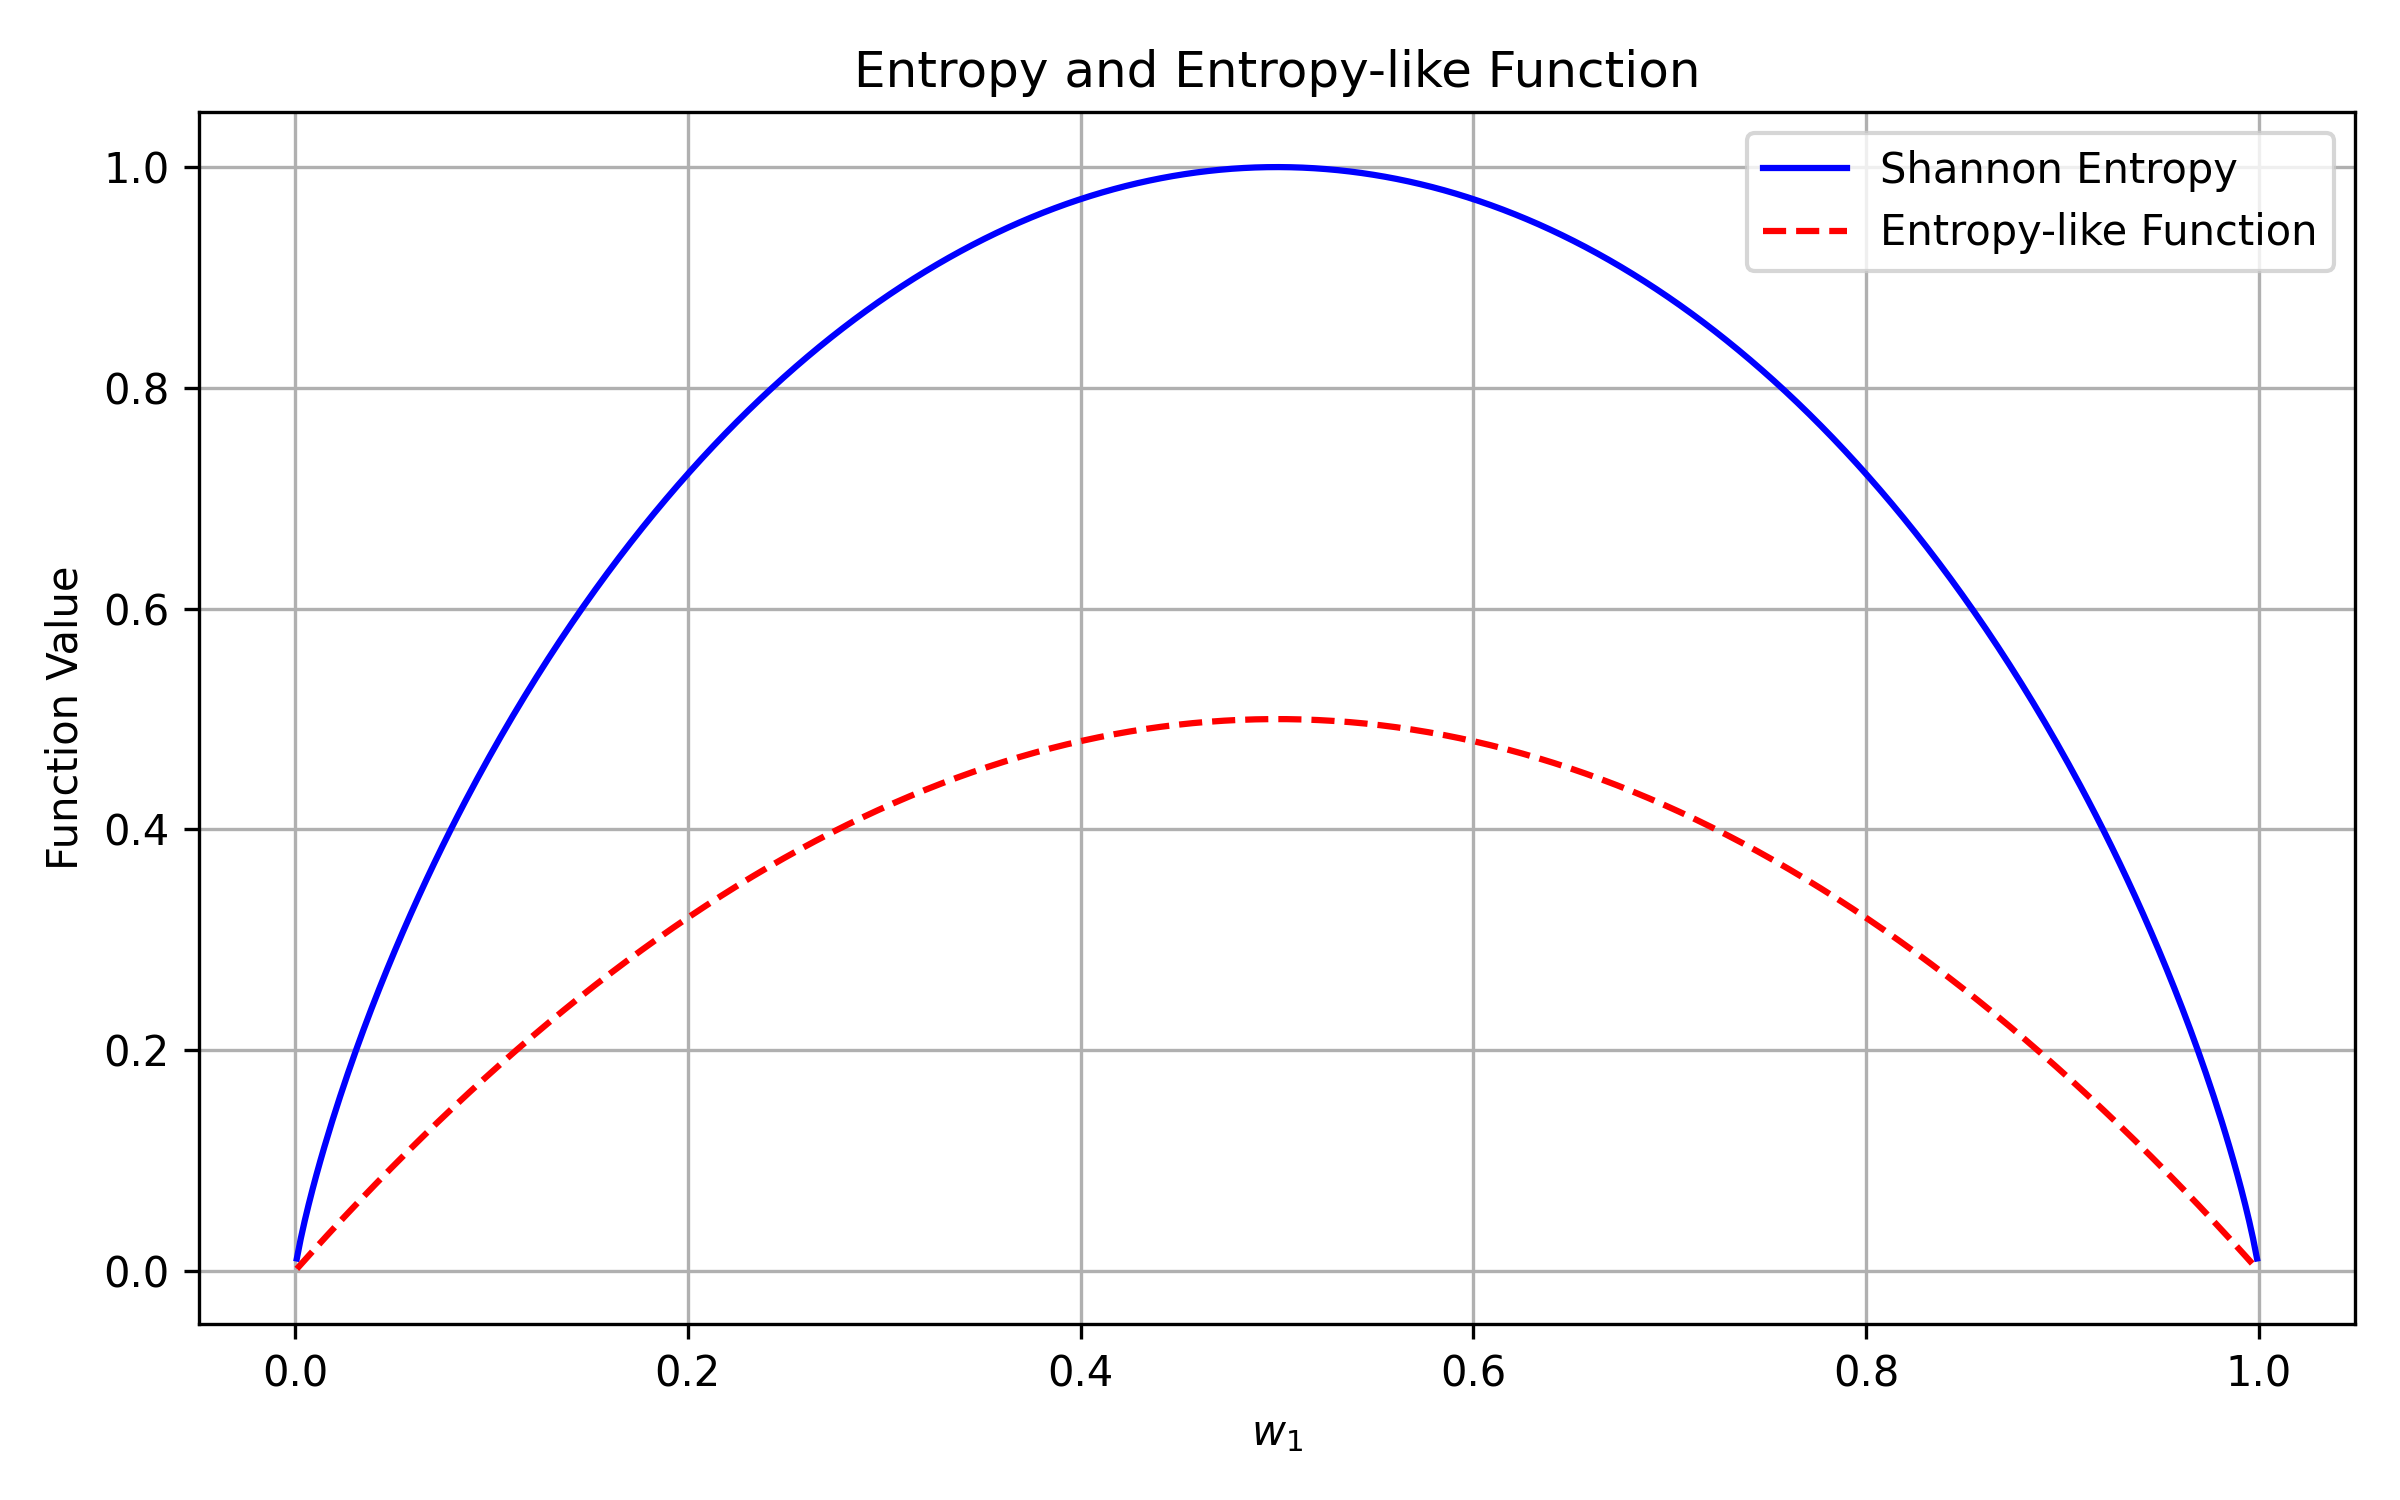
\includegraphics[width=0.8\textwidth]{entropy_plot.png}
\end{center}

همان‌طور که در نمودار مشاهده می‌شود، هر دو تابع در مقدار $w_1 = 0.5$ به بیشینه خود می‌رسند که نشان‌دهنده بیشترین میزان عدم قطعیت یا بیشترین پراکندگی است. در نتیجه می‌توان گفت که آنتروپی و شبه‌آنتروپی هر دو برای سنجش میزان اطلاعات و یکنواختی توزیع کلاس‌ها در مسائل یادگیری ماشین مفید هستند.


	\section*{ سؤال ۲ }
	‫کاربردهاي‬ ‫آنتروپی‬ ‫و‬ ‫انواع‬ ‫آن‬ ‫را‬ ‫با‬ ‫فرمول‬ ‫مربوطه‬ ‫بیان‬ ‫کنید؟‬
	
	\subsection*{پاسخ}
	
	کاربردهای آنتروپی: \\
	
	\begin{itemize}
		\item انتخاب ویژگی در درخت‌های تصمیم 
		\item بهینه‌سازی در یادگیری تقویتی 
		\item ارزیابی مدل‌های طبقه‌بندی
		\item تحلیل خوشه‌بندی
	\end{itemize}
	
	سه نوع آنتروپی که در یادگیری ماشین کاربرد فراوان دارند عبارت‌اند از:
	
	\begin{itemize}
		\item \textbf{آنتروپی شرطی}:
		\begin{align*}
			H(Y|X) &= \sum_x P(x)\, H(Y \mid X = x) \\
			&= \sum_{x \in X} P(x)\left( -\sum_{y \in Y} P(y|x) \log P(y|x) \right) \\
			&= -\sum_{x \in X} P(x) \sum_{y \in Y} P(y|x) \log P(y|x)
		\end{align*}
		
		این مقدار نشان می‌دهد که با دانستن $X$، چقدر عدم قطعیت در مورد $Y$ باقی می‌ماند.
		
		\item \textbf{آنتروپی متقابل (اطلاعات متقابل)}:
		\[
		I(X;Y) = H(Y) - H(Y|X)
		\]
		که مقدار اطلاعات مشترک بین $X$ و $Y$ را نشان می‌دهد. هرچه این مقدار بیشتر باشد، وابستگی متقابل بین دو متغیر بیشتر است.
		
		\item \textbf{فاصله کولبک-لیبلر (KL-Divergence)}:
		\[
		D_{KL}(P \parallel Q) = \sum_{x \in X} P(x) \log \frac{P(x)}{Q(x)}
		\]
		که فاصله بین دو توزیع احتمالاتی $P$ و $Q$ را اندازه می‌گیرد و در آموزش مدل‌هایی مانند Variational Autoencoders کاربرد دارد.
	\end{itemize}
	
	
	
\end{document}